\subsection{Protocol Details}
This section describes the message sequence of BRSKI illustrated in figure \ref{brski-protocol} and elaborates on content of the exchanged messages. The numbering sequence referenced through this section refers to the message numbers in figure \ref{brski-protocol}.

\begin{figure}[htbp]
	\centering
	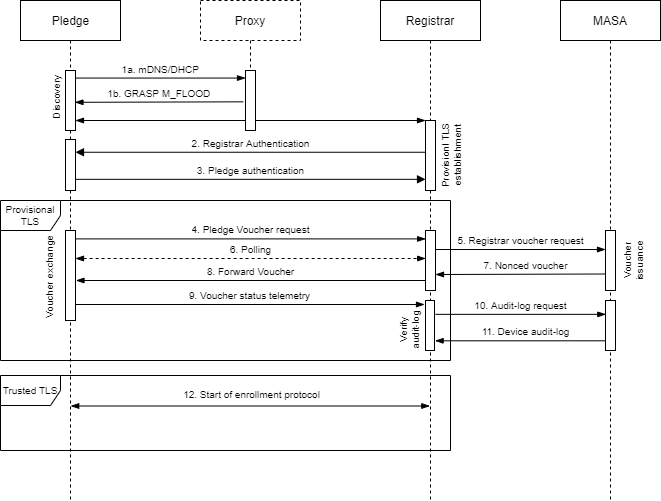
\includegraphics[scale=0.4]{Images/brski-architecture.png}
	\caption{A successful BRSKI protocol run.}
	\label{brski-protocol}
\end{figure}

\begin{itemize}
	\item \textit{Message 1a, 1b (Discovery phase):} It is the first phase of the protocol where the pledge identifies the domain proxy. This can be performed by a pledge initiated mechanism as in message (1a) or via a proxy initiated mechanism as in message (1b). After successful discovery, the pledge can address a domain registrar through the proxy.

	\item \textit{Message 2, 3 (Provisional TLS establishment):} The pledge attempts to establish a TLS channel with each discovered registrar to ensure End-to-End security. The pledge must not use any TLS version lower than TLS 1.2, while TLS 1.3 is the encouraged version to be used. To establish the channel, mutual authentication has to be performed.
	At first, in message (2), the pledge receives the registrar's server certificate. However, the pledge does not posses any trust anchors to verify it yet. Therefore, the pledge accepts the registrar's certificate provisionally.
	Next in message (3), the pledge is authenticated via the installed IDevID. The registrar must be able to verify the provided certificate, however the distribution of the trust anchors for this task is out-of-scope of BRSKI.
	Meaning, the information received by the pledge must be untrusted, although it is in a TLS channel, till a trusted trust anchor to verify the certificate is received. 

	\item \textit{Message 4:} Having established a secure provisional TLS channel, the pledge initiates the voucher exchange by sending a pledge voucher request to the registrar in message (4). The request must contain a unique nonce per bootstrapping attempt to protect against replay attacks. Also, the request contains the `proximity-registrar-cert' and the pledge serial number.
	The `proximity-registrar-cert' is the \gls{ee} certificate of the registrar which is also used to establish the provisional TLS channel. Pledge serial number is a manufacturer defined unique identifier for each device. It is different from the IDevID certificate serial number. Since not all devices have a real-time clock, depending on the device capabilities, the request is recommended to have the 'created-on' value. Finally, the request must be signed using the pledge's IDevID certificate.
	\par
	The registrar authorizes the pledge based on the authenticated information presented in the pledge's IDevID and the registrar's policy. The policy can be either to allow any device from a specific vendor, to allow any device of a specific type, or to allow a specific type of devices from a specific vendor.
	
	\item \textbf{\underline{\textit{Message 5 (Polling):} TODO}}
	
	\item \textit{BRSKI-EST TLS channel:} The registrar initiates a TLS 1.2 or newer channel with the MASA where all subsequent communication between the two parties occur within this secure channel. The MASA URL is obtained from the pledge IDevID, as mentioned earlier. To authenticate the MASA, the registrar should be configurable with trust anchors on a per vendor MASA basis as part of the sales process. Moreover, the registrar should also support client authentication mechanisms such as TLS client certificate, HTTP Basic, Digest, or \gls{scram}; however TLS Client Certificate based authentication is the recommended method.
	
	\item \textit{Message 6:} After obtaining the pledge's voucher request, the registrar constructs a registrar voucher request that is sent to the MASA to obtain a voucher for the pledge. The registrar voucher request is a JSON document that is signed using a CMS structure. The JSON document encapsulates the pledge voucher request CMS object that was sent to the registrar and is referred to as `prior-signed-voucher-request'. Moreover, the request contains the `created-on' field which holds the timestamp the request was formed on. In addition, it consists of other fields which relate to the pledge request like the pledge serial number, the nonce used produced by the pledge and used in the pledge request, and `idevid-issuer' field which holds the issuer value of the pledge IDevID certificate. The registrar includes some certificates in the registrar voucher request CMS object as well. Those certificates are used by the MASA to be pinned into the voucher to be later used by the pledge as a trust anchor for authenticating the domain registrar. Therefore, the certificates enclosed by the registrar in the request have to be part of the chain it wishes the MASA to pin in the voucher. Hence the specificity of the attached certificates is considerably significant. A `pinned-domain-cert' can be as specific as the registrar's TLS \gls{ee} certificate. On the other hand, if it is as general as a public webPKI \gls{ca} it could permit any entity that possess a certificate issued by that authority to claim ownership of the device.
	\par
	
	\textbf{\underline{	In case of nonceless vouchers ...}}
	
	\item \textit{Message 7:} upon receiving the voucher request, the MASA performs a set of checks to decide weather to issue the requested voucher. Given the fact that vouchers have a short lifetime, the request may be from a registrar that has been issued a voucher previously, i.e a voucher renewal request. In this case, the request should be automatically authorized by the MASA.
	\par
	 The MASA extracts the certificate chain attached in the signed CMS object. If the domain CA is unknown to the MASA it is considered as a temporary trust anchor as the intention is not to authenticate the message rather to establish consistency of the domain PKI. According to the MASA's policy, it decides which certificate of the chain supplied by the registrar it chooses to pin. It may be the farthest certificate of the chain, or it may be as close as the \gls{ee} TLS certificate of the registrar. If revocation information is available for that certificate, it must be checked by the MASA to prevent issuance of new or renewed vouchers to unauthorized registrars. Next, the CMS signature is validated using the domain's CA extracted from the voucher request. Also, the signing certificate is verified to contain the `id-kp-cmcRA' Extended Key Usage. This ensures that the signer is an entity that is authorized to be a registrar of the domain. Hence, assures domains that a MASA only accepts requests from domain registrars. 
	 \par
	 In case of nonceless requests, It is mandatory for the MASA to authenticate the registrar.
	 \par 
	 In case of nonced voucher requests, the MASA verifies that the `prior-signed-voucher-request', enclosed in the registrar request, contains a `proximity-registrar-cert' that is coherent to the certificate used to sign the registrar voucher request. Moreover, the nonce is verified to be consistent between the registrar voucher request and the `prior-signed-voucher-request'.
	 \par
	 Subsequent to a successful validation of the request, the MASA responds with an issued voucher in message (6). Any issued voucher by the MASA is recorded in the audit-log. Otherwise if a problem occurs, a response with the appropriate http signaling as described in \cite{brski}. For example, a 403 status code response if the voucher request is not signed correctly, or a 406 status code response if the requested voucher type or algorithms cannot be issued due to the MASA's awareness that such pledge is not capable of processing them.
	 
	\item \textit{Message 8:} The registrar evaluates the received voucher solely for transparency and future audit-log verification. The received voucher is forwarded to the pledge without any interference or modification from the registrar.

	\item \textit{Message 9:}
 	 After the pledge successfully receives a voucher, the pledge must indicate its status regarding the voucher to the domain. This occurs by sending a status message to the registrar. The pledge decides weather to accept the voucher or not through the voucher validation process. If acceptable, the message should contain the version of BRSKI and a boolean status field to indicate the acceptance status. In case of an unacceptable voucher or a failure, the pledge is expected to fail gracefully. The message should contain a Reason field with a string commenting on the cause. Nevertheless, the Reason should not be excessively descriptive as it may be sent to an unauthenticated and potentially malicious registrar.
	 \par
	 Bearing the voucher, the pledge verifies its validity. It verifies the signature using the manufacturer installed MASA trust anchor. It verifies also that the serial number enclosed in the voucher matches its own. For nonced vouchers, the pledge verifies the voucher nonce corresponds to the nonce it sent earlier in the voucher request. However nonceless vouchers can be accepted according to pledge local policy. The pledge can be configured to always accept nonceless vouchers to realize the use case where the MASA is unreachable at the time of pledge deployment.
	 \par
 	 A pledge could be operating in other similar security reduced mode that skip voucher validation in favor of offline or emergency touch-based deployment bootstrapping procedures. For example, \gls{tofu} or physical presence methods such as the use of serial console or depressing a physical button during bootstrapping. However, \gls{tofu} must not be available unless a hardware-assisted \gls{nea} is supported. Meanwhile, it is only recommended for other methods of skipping voucher validation. This recommendation serves as a prevention against unintended use of offline methods when autonomic methods fail or are unavailable.
	 
	\item \textit{Message 10:} After receiving the pledge status telemetry message, the registrar requests the MASA audit-log from the MASA. The log data helps the registrar make a knowledgeable decision regarding further proceeding of the bootstrapping process. The decision making criteria is based upon the security requirements of the registrar domain. Hence, the criteria is out of the protocol's scope.
	The request content is the exact same registrar voucher-request sent earlier to the MASA, but is directed through a different URI specific for requesting the audit log, which is ``/.well-known/brski/requestauditlog". Reusing the same message minimizes the required cryptographic and message operations on both ends. The registrar may reuse the cached voucher request and the MASA may take advantage of its internal state to correlate the message with the already verified request averting additional operations.
	
	\item \textit{Message 11:} 
	A MASA can infer the proper pledge log to be prepared from the ``idevid-issuer" and the ``serial-number" information included in the received request of the previous message. Instead of immediately responding with the audit-log, the MASA can a HTTP 201 ``Created" response with a URL in the ``Location" header field redirecting to actual audit-log. The response log is a JSON format document consisting of all the log entries associated with the pledge. Nevertheless, a MASA that sends out URLS has to ensure they are unpredictable to avoid enumeration attacks against device audit-logs.
	\par
	The log format structure consists of several entries: ``version", ``events", and ``truncation". ``version" is an integer value representing the log format version. ``events" is an array of event objects that are associated to the device. 
	Each of the event objects is comprised of a set of entries. The ``date" entry represents the event's timestamp in the format according to \cite{rfc3339}. 
	The ``domainID" is a unique identifier for the domain's registrar that encodes the pinned-domain-cert's SubjectKeyIdentifier or SPKI fingerprint in base64. A ``nonce", if exists, is a base64 encoding of the same nonce used in the voucher request and issued voucher. If it is a nonceless voucher, then the field should preferably be set to null rather than omitting it. 
	The ``assertion" field indicates the level of verification with which the MASA issued the voucher. It can have one of three values: ``verified", ``logged", and ``proximity"; the latter being the one supoorted by this protocol.
	``truncated" field shows the number of event truncations for the specified domainID.
	Lastly, since audit-logs can be arbitrarily large, duplicated or old entries may be truncated as an optimization for the log structure. The ``truncation" entry contains meta-information about truncated entries such as ``nonced duplicates", ``nonced duplicates", and ``arbitrary".
	\par
	On the pledge side, 
	
	\item \textit{Message 12:} 

	
\end{itemize}









